
\documentclass{beamer}


% THEME
%%%%%%%%%%%%%%%%%%%%%%%%%%%%%%%%%%%%%%%%%%%%%%%%%%%%%%%%%%%%%%%%%%%%%%%%%%%%%%%%


\definecolor{kotlinBgDark}{RGB}{20,52,74}
\definecolor{kotlinBgBright}{RGB}{51,109,146}
\definecolor{slidesBgDark}{RGB}{32,39,41}


% https://www.hartwork.org/beamer-theme-matrix/
\mode<presentation>
{
  \usetheme{Rochester}
  \usecolortheme{seagull}
  \setbeamercolor*{frametitle}{fg=white,bg=kotlinBgBright}
}
% get rid of navigation symbols at the bottom
\setbeamertemplate{navigation symbols}{}


% PACKAGES
%%%%%%%%%%%%%%%%%%%%%%%%%%%%%%%%%%%%%%%%%%%%%%%%%%%%%%%%%%%%%%%%%%%%%%%%%%%%%%%%

\usepackage{color}
\usepackage{xcolor}
\usepackage{listings}
\usepackage{hyperref}

\usepackage{graphicx}
\graphicspath{ {images/} }



% CUSTOM COMMANDS
%%%%%%%%%%%%%%%%%%%%%%%%%%%%%%%%%%%%%%%%%%%%%%%%%%%%%%%%%%%%%%%%%%%%%%%%%%%%%%%%

\makeatletter
    \newenvironment{withoutheadline}{
        \setbeamertemplate{headline}[default]
        \def\beamer@entrycode{\vspace*{-\headheight}}
    }{}
\makeatother


\newcommand\sektion[1]{
  \section{#1}
% http://tex.stackexchange.com/questions/44983/beamer-removing-headline-and-its-space-on-a-single-frame-for-plan-but-keepin
{
\setbeamercolor{frametitle}{bg=slidesBgDark} {
\setbeamercolor{background canvas}{bg=slidesBgDark} {
  \frame{
    \textbf{\huge\textcolor{white}{#1}}
    \noindent\makebox[\linewidth]{\textcolor{kotlinBgBright}{\rule{\paperwidth}{1.4pt}}} % http://tex.stackexchange.com/questions/88502/how-to-change-the-shaded-color-of-the-rule-command
  }}
}
}
}

% LISTING
%%%%%%%%%%%%%%%%%%%%%%%%%%%%%%%%%%%%%%%%%%%%%%%%%%%%%%%%%%%%%%%%%%%%%%%%%%%%%%%%

\definecolor{IJ_text}{RGB}{169,183,198}
\definecolor{IJ_background}{RGB}{43,43,43}
\definecolor{IJ_keyword}{RGB}{204,120,50}
\definecolor{IJ_string}{RGB}{106,135,89}
\definecolor{IJ_comment}{RGB}{128,128,128}
\definecolor{IJ_identifier}{RGB}{255,198,109}

% https://en.wikibooks.org/wiki/LaTeX/Source_Code_Listings
% http://tex.stackexchange.com/questions/28229/extend-a-language-with-additional-keywords
\lstset{language=Java}
\lstset{
 morekeywords={if, else, fun, val, var, get, set}
}
\lstset{%
    backgroundcolor=\color{IJ_background},%
    basicstyle=\color{IJ_text}\ttfamily,
%    basicstyle=\small\ttfamily,%
    keywordstyle=\color{IJ_keyword}\ttfamily,
    stringstyle=\color{IJ_string}\ttfamily,
    commentstyle=\color{IJ_comment}\ttfamily,
% NO! as java vs kotlin issue :( identifierstyle=\color{IJ_identifier}\ttfamily,
    numbers=left, numberstyle=\tiny, stepnumber=1, numbersep=5pt,%
    framexleftmargin=12pt,
}%
%\lstset{framesep=10pt}
%\lstset{xleftmargin=10pt,xrightmargin=10pt}
%\lstset{emph={%  
%    val, var%
%    },emphstyle={\color{red}\bfseries\underbar}%
%}%

\begin{document}

\title{Kotlin Vienna 101}   
\author{Christoph (Leiter $\vert$ Pickl)} 
\date{\today} 

\section{Kotlin 101}
% http://tex.stackexchange.com/questions/44983/beamer-removing-headline-and-its-space-on-a-single-frame-for-plan-but-keepin
{
\setbeamertemplate{footline}{}
\setbeamercolor{frametitle}{bg=slidesBgDark} {
\setbeamercolor{background canvas}{bg=slidesBgDark} {
  \frame{
    
\includegraphics[height=0.6cm]{kotlin_logo_transparent}\textbf{\Huge\textcolor{white}{otlin 101}}
    \noindent\makebox[\linewidth]{\textcolor{kotlinBgBright}{\rule{\paperwidth}{1.4pt}}} % http://tex.stackexchange.com/questions/88502/how-to-change-the-shaded-color-of-the-rule-command
    \vspace{2.0pt} \\
    \textbf{\large{\textcolor{white}{Christoph (Leiter $\vert$ Pickl)}}} \\
    \textbf{\footnotesize{\textcolor{white}{Vienna, Austria -- June 20, 2016}}}
  }
}
}
}



\fullimageCapt{lighthouse}{A lighthouse on \href{https://en.wikipedia.org/wiki/Kotlin_Island}{Kotlin Island}, Russia}{}

\sektion{Introduction}

\frame{\frametitle{Language fundamentals} 
  \begin{itemize}[<+->]
    \item Statically typed, \textbf{hybrid} programming language for the \textbf{JVM}
    \item Fully \textbf{interoperable} with Java
    \item Runs on \textbf{Android} (generates 1.6 bytecode)
    \item Possibility to compile to \textbf{JavaScript}
    \item Focuses on \textbf{industry}, tooling and safety
    \item \textbf{Open source} compiler and tools (Apache 2 license)
  \end{itemize}
}

\frame{\frametitle{Historic abstract} 
  \begin{itemize}[<+->]
    \item Developed by \textbf{JetBrains} (IntelliJ, ReSharper, WebStorm, \ldots)
    \item Development already started \textbf{2010}
    \item Since then used in \textbf{projects} at JetBrains, Prezi and Expedia
    \item 2M+ LoC and 100+ contributers at \textbf{GitHub}
    \item \href{https://blog.jetbrains.com/kotlin/2016/02/kotlin-1-0-released-pragmatic-language-for-jvm-and-android/}{Version 1.0} released February, 2016
  \end{itemize}

\vspace{10.0pt}

\begin{figure}[h]
\centering
  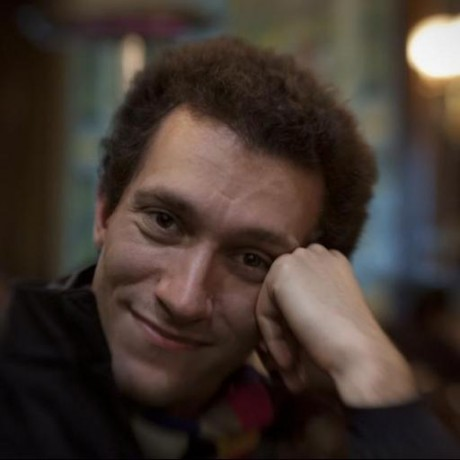
\includegraphics[height=2.0cm]{andrey}
  \vspace{-10.0pt}
  \caption{Andrey Breslav}
\end{figure}
}


\frame{\frametitle{Yet another JVM language?}
\pause
\begin{figure}[h]
  \centering
  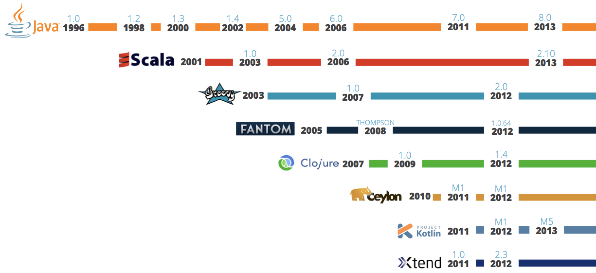
\includegraphics[width=10cm]{jvm_languages}
  \vspace{-10.0pt}
  \caption{Source: \href{https://zeroturnaround.com/rebellabs/the-adventurous-developers-guide-to-jvm-languages-java-scala-groovy-fantom-clojure-ceylon-kotlin-xtend/}{RebelLabs}}
\end{figure}
}

\frame{\frametitle{Java is dead, long live Java}
\pause
\quotes{Most people talk about Java the language, and this may sound odd coming from me, but I could hardly care less. \\ At the core of the Java ecosystem is the JVM.}\pause
\textbf{\small{James Gosling,}}\\
\textbf{\tiny{Creator of the Java Programming Language (2011, TheServerSide)}}
}

\fullimage{java_no_cool}

\frame{\frametitle{Yet another JVM language!}
  \begin{itemize}[<+->]
    \item Well known company with good \textbf{tooling} support
    \item It got nothing new, just the \textbf{best of all} of them
    \item It's about the \textbf{ecosystem}, not the language
    \begin{itemize}
       \item \textit{Empirical Analysis of Programming Language Adoption} (\href{http://sns.cs.princeton.edu/docs/asr-oopsla13.pdf}{PDF})
    \end{itemize}
    \item It's really, really easy to \textbf{learn}
    \begin{itemize}
        \item ``\textit{Scala for \sout{dummies} the masses}''
    \end{itemize}

  \end{itemize}
}
\sektion{Language Features}

\frame{\frametitle{We'll have a look at \ldots}
\begin{enumerate}
	\item Type inference
	\item Function declaration
	\item Lambdas
	\item Null handling
	\item Smart casts
	\item Properties
	\item Extension methods
	\item  Named \& default parameters
	\item Data classes
	\item Collection API
\end{enumerate}
}

%%%%%%%%%%%%%%%%%%%%%%%%%%%%%%%%%%%%%%%%%%%%%%%%%%%%%%%%%%%%%%%%%%%%%%%%%%%%%%%%
\begin{frame}[fragile] \frametitle{Type inference}
\begin{lstlisting}
// mutable variable of type Int
var x = 42

// immutable value of type String
val y = "foobar"

// explicit type declaration
val z: Double = 13.37

// whatever the return type is
val z = someFunction()
\end{lstlisting}
\end{frame}


%%%%%%%%%%%%%%%%%%%%%%%%%%%%%%%%%%%%%%%%%%%%%%%%%%%%%%%%%%%%%%%%%%%%%%%%%%%%%%%%
\begin{frame}[fragile] \frametitle{Function declaration}
\begin{lstlisting}
// global function with explicit return type
fun add1(x: Int, y: Int): Int {
  return x + y
}

// compact one-line syntax
fun add2(x: Int, y: Int) = x + y
\end{lstlisting}
\end{frame}


%%%%%%%%%%%%%%%%%%%%%%%%%%%%%%%%%%%%%%%%%%%%%%%%%%%%%%%%%%%%%%%%%%%%%%%%%%%%%%%%
\begin{frame}[fragile] \frametitle{Class declaration}
\begin{lstlisting}
// single ctor is initializing its fields
class Greeter(private val prefix: String) {

  // string interpolation, no concatenation
  fun greet(name: String) =
    "$prefix ${name}!"
}
\end{lstlisting}
\end{frame}


%%%%%%%%%%%%%%%%%%%%%%%%%%%%%%%%%%%%%%%%%%%%%%%%%%%%%%%%%%%%%%%%%%%%%%%%%%%%%%%%
\begin{frame}[fragile] \frametitle{A simple application}
\begin{lstlisting}
fun main(args: Array<String>) {
  // no "new" keyword necessary
  val greeter = Greeter("Hello")

  // prints: "Hello sIT!"
  println(greeter.greet("sIT"))
}
\end{lstlisting}
\end{frame}

%%%%%%%%%%%%%%%%%%%%%%%%%%%%%%%%%%%%%%%%%%%%%%%%%%%%%%%%%%%%%%%%%%%%%%%%%%%%%%%%
\begin{frame}[fragile] \frametitle{Lambdas}
\begin{lstlisting}
TODO
\end{lstlisting}
\end{frame}

%%%%%%%%%%%%%%%%%%%%%%%%%%%%%%%%%%%%%%%%%%%%%%%%%%%%%%%%%%%%%%%%%%%%%%%%%%%%%%%%
\begin{frame}[fragile] \frametitle{Null handling}
\begin{lstlisting}
val maybe: String? = ...

maybe.length // COMPILE ERROR!!!

maybe?.length // type is Int?
maybe?.length ?: -1 // type is Int
maybe!!.length // i dont f*cking care!

if (maybe != null) {
  maybe.length // smart cast to String
}
\end{lstlisting}
\end{frame}


\fullimage{its_beautiful}

%%%%%%%%%%%%%%%%%%%%%%%%%%%%%%%%%%%%%%%%%%%%%%%%%%%%%%%%%%%%%%%%%%%%%%%%%%%%%%%%

\begin{frame}[fragile]
\frametitle{Smart casts}
\begin{columns}[t]
\begin{column}{0.5\textwidth}
\begin{center}
  Java
\end{center}
\begin{lstlisting}[style=twosided]
Object x = ...;
if (x instanceof A) {
  a = (A) x;
  a.foo();
} else if (x instanceof B) {
  B b = (B) x;
  b.bar();
} else {
  throw new Exception("Sad panda!");
}
\end{lstlisting}

\end{column}
\begin{column}{0.5\textwidth}
\begin{center}
  Kotlin
\end{center}
\begin{lstlisting}[style=twosided]
interface A { fun foo() }
interface B { fun bar() }
// ----------------------

val x: Any = ...
when (x) {
  is A -> x.foo()
  is B -> x.bar()
  else -> throw Exception("Sad panda!")
}
\end{lstlisting}
\end{column}
\end{columns}
\end{frame}

%%%%%%%%%%%%%%%%%%%%%%%%%%%%%%%%%%%%%%%%%%%%%%%%%%%%%%%%%%%%%%%%%%%%%%%%%%%%%%%%

\begin{frame}[fragile] \frametitle{Enum safety -- Java approach}
\begin{lstlisting}[basicstyle=\color{IJ_text}\ttfamily\tiny]
public enum SignMode {
  TAC {
    @Override public <T> T callback(Callback<T> callback) {
      return callback.onTac(); }},
  CARD_TAN {
    @Override public <T> T callback(Callback<T> callback) {
      return callback.onCardTan(); }},
  TAN {
    @Override public <T> T callback(Callback<T> callback) {
      return callback.onTan(); }};

  public abstract <T> T callback(Callback<T> callback);

  public interface Callback<T> {
    T onTac();
    T onCardTan();
    T onTan();
  }
}

\end{lstlisting}
\end{frame}

\begin{frame}[fragile]
\frametitle{Enum safety -- compared}
\begin{columns}[t]
\begin{column}{0.5\textwidth}
\begin{center}
  Java
\end{center}
\begin{lstlisting}[style=twosided]
public int mode2int(SignMode mode) {
  return mode.callback(
  new Callback<Integer>() {
  @Override public Integer onTac() {
    return 1;
  }
  @Override public Integer onCardTan() {
    return 2;
  }
  @Override public Integer onTan() {
    return 3;
  }
  });
}
\end{lstlisting}
\end{column}
\begin{column}{0.5\textwidth}
\begin{center}
  Kotlin
\end{center}
\begin{lstlisting}[style=twosided]
enum class SignMode {
  TAC, CARD_TAN, TAN
}

fun mode2int(mode: SignMode) =
  when(mode) {
    SignMode.TAC -> 1
    SignMode.CARD_TAN -> 2
    SignMode.TAN -> 3
    // COMPILE ERROR if branch missing
  }
\end{lstlisting}
\end{column}
\end{columns}
\end{frame}



%%%%%%%%%%%%%%%%%%%%%%%%%%%%%%%%%%%%%%%%%%%%%%%%%%%%%%%%%%%%%%%%%%%%%%%%%%%%%%%%
\begin{frame}[fragile] \frametitle{Properties}
\begin{lstlisting}
TODO
\end{lstlisting}
\end{frame}


%%%%%%%%%%%%%%%%%%%%%%%%%%%%%%%%%%%%%%%%%%%%%%%%%%%%%%%%%%%%%%%%%%%%%%%%%%%%%%%%
\begin{frame}[fragile] \frametitle{Extension methods}
\begin{lstlisting}
TODO
\end{lstlisting}
\end{frame}


%%%%%%%%%%%%%%%%%%%%%%%%%%%%%%%%%%%%%%%%%%%%%%%%%%%%%%%%%%%%%%%%%%%%%%%%%%%%%%%%
\begin{frame}[fragile] \frametitle{Named \& default parameters}
\begin{lstlisting}
TODO
\end{lstlisting}
\end{frame}


%%%%%%%%%%%%%%%%%%%%%%%%%%%%%%%%%%%%%%%%%%%%%%%%%%%%%%%%%%%%%%%%%%%%%%%%%%%%%%%%

\begin{frame}[fragile]
\frametitle{Data classes}
\begin{columns}[t]
\begin{column}{0.5\textwidth}
\begin{center}
  Java
\end{center}
\begin{lstlisting}[style=twosided]
public class Person {
 private final String name;
 private final int age;
 public Person(String name, int age) {
  this.name = name;
  this.age = age;
 }
 public String getName() {
  return name;
 }
 public int getAge() {
  return age;
 }
 public boolean equals(Object other) {
  ...
 }
 public int hashCode() {
  ...
 }
 public String toString() {
  ...
 }
}
\end{lstlisting}

\end{column}
\begin{column}{0.5\textwidth}
\begin{center}
  Kotlin
\end{center}
\begin{lstlisting}[style=twosided]
data class Person(
 val name: String,
 val age: Int
)

// same as with lombok but better ;)

// primary ctor deals with getters
// and field initialisation

// generates equals/hashCode/toString
// and a copy function (no builders!)
\end{lstlisting}
\end{column}
\end{columns}
\end{frame}


%%%%%%%%%%%%%%%%%%%%%%%%%%%%%%%%%%%%%%%%%%%%%%%%%%%%%%%%%%%%%%%%%%%%%%%%%%%%%%%%
\begin{frame}[fragile] \frametitle{Collection API}
\begin{lstlisting}
TODO
\end{lstlisting}
\end{frame}


%%%%%%%%%%%%%%%%%%%%%%%%%%%%%%%%%%%%%%%%%%%%%%%%%%%%%%%%%%%%%%%%%%%%%%%%%%%%%%%%
\frame{\frametitle{Further Features}
\begin{itemize}
	\item Delegation
	\item String handling
	\item Sealed classes
	\item Pattern matching
	\item Operator overloading
	\item == as equals
	\item \texttt{if} and \texttt{when} as an expression
	\item Rename imports
	\item Backticks for escaping
	\item \ldots and much much more \ldots
\end{itemize}
}

\sektion{Epilog}

\frame{\frametitle{Summary} 
\begin{itemize}
	\item Its good
	\item Yes it is
\end{itemize}
}


\end{document}
